
\section{Deformation of the drops}
\label{ap:deformation} 

Bubbles or droplets with a high Bond number are known to undergo significant deformations, and these deformations can significantly influence their rising velocity \citep{bunner2003effect,tripathi2014}. 
This appendix is dedicated to assessing the deformation of fluid inclusions within the range of dimensionless parameters prescribed in the main-body of the article. 
It is demonstrated that, across this entire range, the deformation remains small. 
Axisymmetric fluid inclusions are characterized by their aspect ratio, defined as the ratio of their cross-stream axis to the axis parallel to their velocity. 
However, for three-dimensional configurations involving deforming fluid inclusions, the definition of the aspect ratio becomes impractical due to the loss of symmetry in deformations \citep{bunner2003effect}. 
Consequently, to examine the shape of a given particle, we introduce its aspect ratio  
\begin{equation}
    \chi =  \sqrt{I_1 /I_2},
\end{equation}
with $I_1$ and $I_2$, the maximum and minimum eigenvalues of the particle inertia tensor defined as
\begin{equation*}
    \textbf{I}
    = \int_{V} \left[
        (\textbf{r}\cdot \textbf{r}) \bm\delta  - \textbf{rr}
        \right]
    d\textbf{x}.
\end{equation*}
Here, $\bm\delta$ is the unit tensor, $V$ the volume of a given particle and $\textbf{r} = \textbf{x} - \textbf{x}_i$, with $\textbf{x}_i$ is the center of mass of the fluid inclusion. 
Then, $\chi_p$ which is the averaged value of $\chi$ over all particles and timesteps, gives us a reliable way to compute the mean deformation of droplets. 
This definition has been used to characterize the deformation and orientation of rising bubbles \citep{bunner2003effect}. 
\begin{figure}[h!]
    \centering
    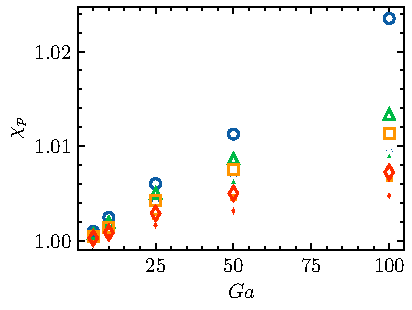
\includegraphics[height = 0.3\textwidth]{image/HOMOGENEOUS_NEW/PA/chi.pdf}
    \caption{Mean aspect ratio of the droplets $\chi_p$, as a function of the \textit{Galileo} number, and the volume faction $\phi$,  for two different viscosity ratios.  
    The symbols correspond to different volume fraction ($\pmb\bigcirc$) $\phi = 0.01$; ($\pmb\triangle$) $ \phi = 0.05$; ($\pmb\square$) $\phi = 0.1$ ($\pmb\lozenge$) $\phi = 0.2$.
    The hollow symbols correspond to $\lambda = 1$, the filled symbols to $\lambda = 10$.
    }
    \label{fig:chi}
\end{figure}
\ref{fig:chi} displays the values of $\chi_p$ as a function of $Ga$.
As depicted in this figure, it is evident that droplets undergo flattening as $Ga$ increases and the drop volume fraction decreases. 
Additionally, it appears that, for lower viscosity ratios, the droplets exhibit a lower aspect ratio compared to more viscous drops.
In the low $Ga$ range, the average aspect ratio $\chi_p$ tends towards $1$, implying that in this regime droplets are mainly spherical. 
In summary, we observe a maximum $\chi_p$ value of $1.02$, which implies a deviation from a spherical shape of about $2\%$.

%\begin{figure}[h!]
%  \centering
%  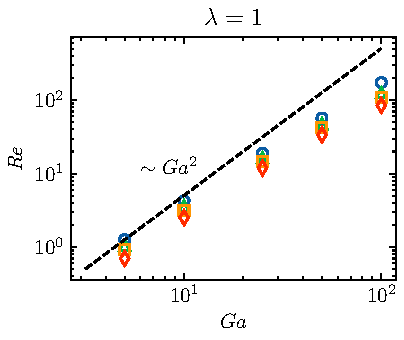
\includegraphics[height = 0.3\textwidth]{image/HOMOGENEOUS_NEW/CA/Re_l_1.pdf}
%  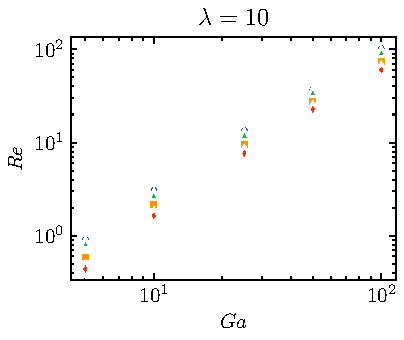
\includegraphics[height = 0.3\textwidth]{image/HOMOGENEOUS_NEW/CA/Re_l_10.pdf}
%  \caption{
%      Averaged Reynolds number based on the averaged relative velocity, $Re = \rho_fU d /\mu_f$, with $U = |<\textbf{u}_d> - <\textbf{u}_d>|$.
%      $<\textbf{u}_d>$ and $<\textbf{u}_c>$ are the volume time averaged dispersed and continuous velocity respectively.
%  }
%  \label{fig:Reall}
%\end{figure}

% \begin{table}  
% \begin{tabular}{c|c|c|c|l}
%  calls  &  total  &   self  & \% total  & function \\ \hline
%  10636901 &  4861.39 &  4861.39  &   31.8\% (28.4\% - 36.7\%) &   mpi\_boundary\_level():grid/multigrid-mpi.h:83\\
%     53604 &  3097.64 &  1988.97  &   13.0\% (10.8\% - 14.7\%) &   project():poisson.h:501\\
%     26802 &  2022.99 &  1236.57  &    8.1\% ( 7.3\% -  8.8\%) &   viscosity():viscosity.h:173\\
%    107208 &  1984.59 &  1223.33  &    8.0\% ( 6.9\% -  8.9\%) &   heights():heights.h:281\\
%     26802 &  2499.81 &  1099.66  &    7.2\% ( 6.1\% -  7.9\%) &   vof\_0():vof.h:365\\
%   3155070 &  983.66  & 983.66    &  6.4\% ( 3.9\% -  9.1\%)   & mpi\_all\_reduce0():common.h:683\\
%     26802 &  2372.23 &  896.09   &   5.9\% ( 5.1\% -  6.5\%)  &  advection\_term():navier-stokes/centered.h:323\\
%     26802 &  1583.59 &  645.89   &   4.2\% ( 4.1\% -  4.3\%)  &  no\_coalescence():./no-coalescence.h:419\\
%      2681 &  584.39  & 372.15    &  2.4\% ( 2.4\% -  2.5\%)   & track\_bub():RS.c:124\\
%    321624 &  546.74  & 340.36    &  2.2\% ( 1.8\% -  2.6\%)   & reconstruction():fractions.h:476\\
%    107208 &  2777.30 &  303.23   &   2.0\% ( 1.6\% -  2.4\%)  &  curvature():curvature.h:621\\
%     69275 &  992.44  & 254.14    &  1.7\% ( 1.4\% -  1.8\%)   & tag():tag.h:268\\
%     26802 &  328.67  & 202.85    &  1.3\% ( 1.1\% -  1.5\%)   & acceleration\_0():iforce.h:133\\
%     26802 &  2257.27 &  178.19   &   1.2\% ( 0.8\% -  1.3\%)  &  projection():navier-stokes/centered.h:430\\
  %    26802 &  2142.30 &  119.30   &   0.8\% ( 0.5\% -  0.9\%)  &  viscous\_term():navier-stokes/centered.h:362\\
  %    26802 &  145.95  & 116.09    &  0.8\% ( 0.5\% -  0.9\%)   & acceleration\_2():RS.c:166\\
  %    26803 &  111.60  & 111.57    &  0.7\% ( 0.5\% -  0.8\%)   & properties\_0():two-phase-generic.h:101\\
  %    26802 &  172.09  & 100.18    &  0.7\% ( 0.5\% -  0.8\%)   & acceleration():navier-stokes/centered.h:386\\
  %    69275 &   68.91  &  68.88    &  0.5\% ( 0.4\% -  0.5\%)   & z\_indexing():grid/multigrid-mpi.h:145\\
  %      118 &   59.59  &  59.59    &  0.4\% ( 0.2\% -  0.8\%)   & compose\_image():view.h:409\\
  %    26802 &   64.69  &  34.48    &  0.2\% ( 0.2\% -  0.3\%)   & tracer\_advection\_1():./no-coalescence.h:446\\
  %       59 &  129.57  &  28.81    &  0.2\% ( 0.1\% -  0.2\%)   & movies():RS.c:244\\
  %    26803 &   92.48  &  27.24    &  0.2\% ( 0.1\% -  0.2\%)   & stability\_1():tension.h:64\\
  %    26803 &   24.42  &  21.33    &  0.1\% ( 0.1\% -  0.1\%)   & stability():navier-stokes/centered.h:226\\
  % 43894361 &  3001.24 &    5.50   &   0.0\% ( 0.0\% -  0.0\%)  &  boundary\_internal():grid/cartesian-common.h:450\\
  % 42061052 &   25.50  &   3.61    &  0.0\% ( 0.0\% -  0.0\%)   & interpolate():grid/cartesian-common.h:815\\
  %      472 &    2.31  &   2.31    &  0.0\% ( 0.0\% -  0.0\%)   & draw\_vof():draw.h:1052\\
  %    58554 &   25.92  &   0.87    &  0.0\% ( 0.0\% -  0.0\%)   & reduce\_bubbles():./no-coalescence.h:158\\
  %        1 &  15287.89&     0.73  &    0.0\% ( 0.0\% -  0.0\%) &   run():run.h:37\\
  %        1 &    0.28  &   0.28    &  0.0\% ( 0.0\% -  0.0\%)   & init\_0():RS.c:149\\
  %    26802 &  2777.57 &    0.27   &   0.0\% ( 0.0\% -  0.0\%)  &  acceleration\_1():tension.h:94\\
  %      236 &   38.81  &   0.21    &  0.0\% ( 0.0\% -  0.0\%)   & squares():draw.h:1375\\
    %    118 &   59.64  &   0.05    &  0.0\% ( 0.0\% -  0.1\%)   & save():view.h:529\\
    %  63404 &    0.06  &   0.03    &  0.0\% ( 0.0\% -  0.0\%)   & interpolate():grid/cartesian-common.h:816\\
    %      1 &    0.02  &   0.02    &  0.0\% ( 0.0\% -  0.0\%)   & defaults\_3():iforce.h:38\\
    %      1 &    0.01  &   0.01    &  0.0\% ( 0.0\% -  0.0\%)   & defaults\_2():two-phase-generic.h:26\\
    %  26802 &  1583.60 &    0.01   &   0.0\% ( 0.0\% -  0.0\%)  &  vof\_1():./no-coalescence.h:430\\
    %  26802 &    0.01  &   0.01    &  0.0\% ( 0.0\% -  0.0\%)   & set\_dtmax():navier-stokes/centered.h:222\\
    %  26803 &    0.00  &   0.00    &  0.0\% ( 0.0\% -  0.0\%)   & stability\_0():vof.h:143\\
    %      1 &    0.25  &   0.00    &  0.0\% ( 0.0\% -  0.0\%)   & init():navier-stokes/centered.h:213\\
    %      1 &    0.00  &   0.00    &  0.0\% ( 0.0\% -  0.0\%)   & defaults\_0():navier-stokes/centered.h:181\\
    %      1 &    0.00  &   0.00    &  0.0\% ( 0.0\% -  0.0\%)   & restore():output.h:1169\\
    %      1 &    0.00  &   0.00    &  0.0\% ( 0.0\% -  0.0\%)   & cleanup():run.h:52\\
    %      1 &    0.00  &   0.00    &  0.0\% ( 0.0\% -  0.0\%)   & defaults():run.h:44\\
    %      1 &    0.00  &   0.00    &  0.0\% ( 0.0\% -  0.0\%)   & defaults\_4():./no-coalescence.h:483\\
    %      1 &    0.00  &   0.00    &  0.0\% ( 0.0\% -  0.0\%)   & defaults\_1():vof.h:134\\
    %      1 &    0.00  &   0.00    &  0.0\% ( 0.0\% -  0.0\%)   & cleanup\_0():./no-coalescence.h:458\\
    %      1 &    0.00  &   0.00    &  0.0\% ( 0.0\% -  0.0\%)   & default\_display():navier-stokes/centered.h:188\\
    %      1 &    0.00  &   0.00    &  0.0\% ( 0.0\% -  0.0\%)   & stop():RS.c:272\\
% \end{tabular}
% \caption{Profiling of the time taken by functions during the simulation for the parameters.
% Dimensionless parameters of the simulation : 
% $Ga = 25$, $\lambda = 1$, $Bo = 1$, $\zeta = 1.11$ and $\phi = 0.2$.
% Numerical parameters :  $N_b = 125$, $d/\Delta = 37.149$.
% This simulation has been performed on $216$ processors.  }
% \label{tab:performance}
% \end{table}


